%!TEX root = thesis.tex

\chapter{I-POMDPs for Object Detection}
\label{ch:IPOMDP}
The problem of object detection can be formulated as an I-POMDP using the game ``Where's Waldo?'' as an example. This example is presented in \cite{Butko2010b}. The goal of the game is to find a person, Waldo, in an illustrated image full of people and objects that have similar appearance as Waldo himself. For the evaluation we assume we have a detector that recognizes Waldo but the people and objects that are similar to Waldo act as noise in the detector.

From the agent's point of view, the goal in the ``Where's Waldo?'' game is to find Waldo in an image by fixating on different parts of the image using as few fixations as possible. To accomplish that the agent needs to learn a good policy. The policy determines which part of the image the agent fixates on in every time step and the number of fixations needed to find Waldo gives a measure of how well the policy performs. The part of the image that Waldo occupies is the state of the world and we assume that Waldo doesn't move so the state never changes. The agent's belief for each state is  the probability of Waldo being in that state, i.e. positioned in that part of the image, given previous observations and actions.

In this chapter we describe the problem specific models that were implemented and used for evaluation of the ``Where's Waldo?'' problem.

\section{Observation Model}
\label{sec:ObservationModelImpl}
Two different observation models are used for the evaluation. The first one is a model where the agent's ability to distinguish between a signal from an object and noise decays exponentially from the point where the agent is focusing. This observation model is
\begin{equation}\label{eq:ObservationModel}
  \begin{split}
    O_t^j &= \delta (S_t, j) d_{j,k} + Z_t^j \\
          &= \begin{cases}
                d_{j,k} + Z_t^j & \text{if $S_t = j$}\\
                Z_t^j           & \text{otherwise}
             \end{cases}
  \end{split}
\end{equation}
where $Z_t^j$ is zero mean, unit variance Gaussian random noise (i.e. white noise) and
\begin{equation}
  d_{j,k} = 3 \cdot e^{-dist(j,k)}
\end{equation}
where $dist(j,k)$ is the Euclidean distance between locations $j$ and $k$.

We will call this model the \emph{Exponential model}. An example of how this vision system sees an image (without noise) can be seen in Figure \ref{fig:ObsmodelExp}.

\begin{figure}[!htp]
  \centering
  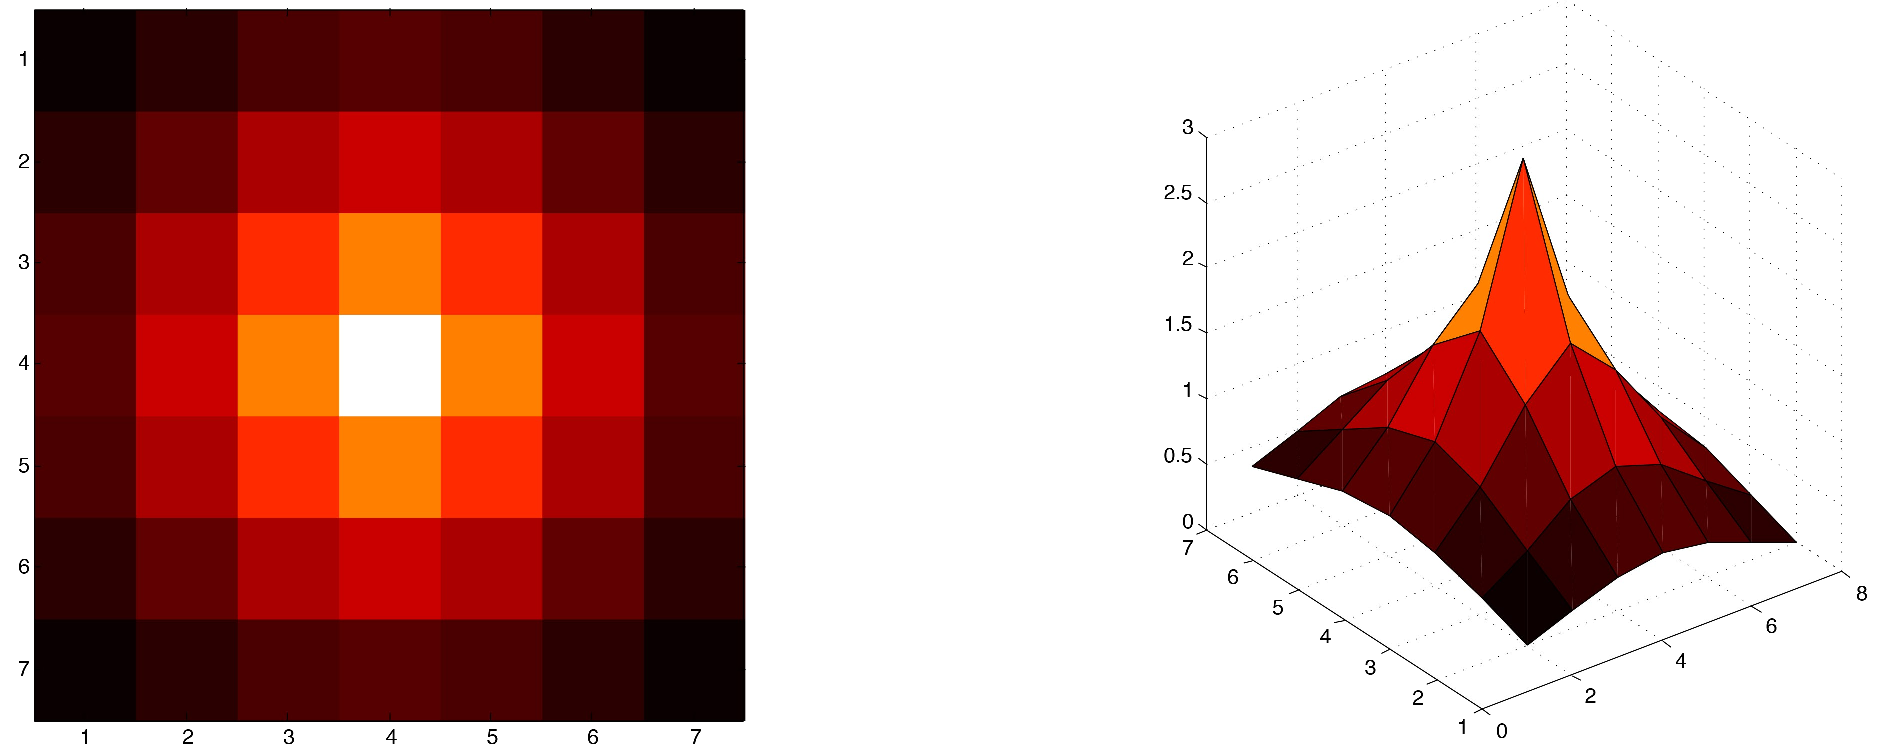
\includegraphics[width=1\textwidth]{figures/obsmodel_exp}
  \caption{A vision system with an exponential decay of focus. The agent focuses on the center of the image and the the focus point is the most reliable one. The ability to distinguish between noise and a signal from an object decreases with the distance from the agent's focus point.}
  \label{fig:ObsmodelExp}
\end{figure}

The second model is a model of the properties of the human eye. This model takes the same form as the exponential model in equation \eqref{eq:ObservationModel} but now $d_{j,k}$ is as described in \cite{Najemnik2005}.

We will call this model the \emph{Human eye model}. An example of how this vision system sees an image (without noise) can be seen in Figure \ref{fig:ObsmodelCont}.

\begin{figure}[!htp]
  \centering
  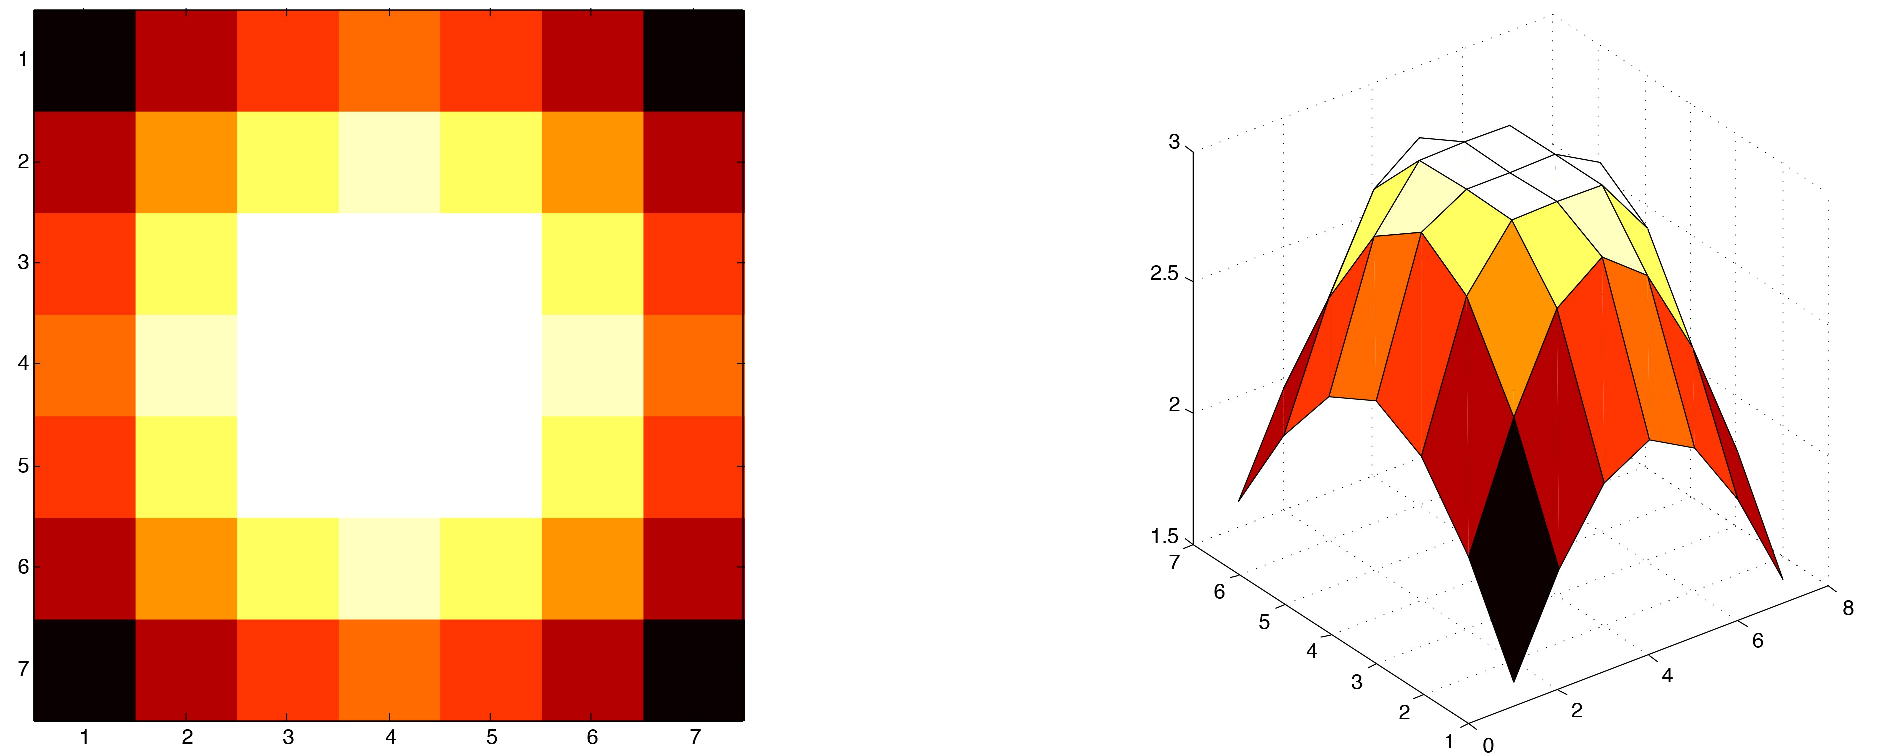
\includegraphics[width=1\textwidth]{figures/obsmodel_cont}
  \caption{A vision system with the characteristics modeled after the human eye. The agent focuses on the center of the image and is able to distinguish between noise and a signal from an object in and around the center. The reliability of the vision drops dramatically in locations further away from the agent's focus point.}
  \label{fig:ObsmodelCont}
\end{figure}

\section{Observation Likelihood}
\label{sec:ObservationLikelihoodImpl}
We assume that given an image, individual observations (i.e. each pixel or cell)
\begin{equation}
  o_t = (o_t^1, \dotsc, o_t^{|\mathcal{S}|})
\end{equation}
are conditionally independent. Then we can write the probability of an observation as
\begin{subequations}
  \begin{align}
    p(o_t | S_t = i, A_t = k) 
      &= \prod_j p(o_t^j | S_t = i, A_t = k) \\
      &= p(o_t^i | S_t = i, A_t = k) \prod_{j \neq i} p(o_t^j | S_t = i, A_t = k) \\
      \intertext{Given the observation model from equation \eqref{eq:ObservationModel} we get}
      &= \gaussianexp{o_t^i - d_{i,k}} \prod_{j \neq i} \gaussianexp{o_t^j} \\
      &= \frac{1}{\sqrt{2\pi}} \frac{\gaussianexppart{o_t^i - d_{i,k}}}{\gaussianexppart{o_t^i}} \prod_j \gaussianexp{o_t^j} \\
      &= \frac{\gaussianexppart{o_t^i - d_{i,k}}}{\gaussianexppart{o_t^i}} Z \\
      &= \exp((o_t^i - \frac{d_{i,k}}{2}) d_{i,k}) K
  \end{align}
\end{subequations}
where $K$ is a constant. Ignoring the constant $K$ and terms not containing $o_t^i$ we can write
\begin{equation}
\label{eq:ProportionalObservationLikelihood}
  p(o_t | S_t = i, A_t = k) \propto \exp{(d_{i,k} o_t^i)}
\end{equation}
and this is the way the observation likelihood has been implemented.

\section{Proportional Belief Updates}
\label{sec:ProportinalBeliefUpdates}
We can combine equation \eqref{eq:UpdateBeliefFixedTarget} for the belief updates with equation \eqref{eq:ProportionalObservationLikelihood} for the proportional observation likelihood and then we get
\begin{equation}
  b_{t+1}^i \propto \exp{(d_{i,k} o_t^i)} b_t^i
\end{equation}
which enables us to calculate the updated belief proportionally. The belief vector can then be normalized after every update to make sure 
\begin{equation}
  \sum_i{b_{t+1}^i} = 1
\end{equation}
holds.
